\documentclass[14pt]{extarticle}
\usepackage{amsmath}
\usepackage{amssymb}
%\usepackage{tikz}
%\usetikzlibrary{calc}
%\usetikzlibrary{trees}
\usepackage{hyperref}
\usepackage{graphicx}
\graphicspath{ {../../chap10/} }
\usepackage[top=0.75in, bottom=0.75in, left=0.75in, right=0.75in]{geometry}
%\newcommand*{\Scale}[2][4]{\scalebox{#1}{\ensuremath{#2}}}%
\usepackage[shortlabels]{enumitem}
\usepackage[most]{tcolorbox}
\definecolor{bg}{RGB}{255,249,227}
% \usepackage{showframe}

\title{\vspace{-5ex}Math 208 Section 10.7}
\date{\vspace{-10ex}}
\usepackage{multicol}
\setlength{\columnsep}{1cm}
\setlength{\parindent}{0pt}
\usepackage{parskip}
\setlength{\parskip}{10pt} % 1ex plus 0.5ex minus 0.2ex}
%\usepackage{ragged2e}


\begin{document}
	\maketitle
	
\section{Homework, Reading, and Other}
\begin{itemize}
	\item Section 10.4
	\item Section 10.7
\end{itemize}

\section{Goals}
\begin{itemize}
	\item Understand and apply rates of change
	\item Evaluate  and interpret elasticity of demand
\end{itemize}

\section{Section 10.7:  Elasticity of Demand}
\subsection{Introduction}
Increasing the price of a product changes the revenue for the seller in a couple of ways.
\begin{itemize}
	\item If demand holds steady (i.e. the seller is able to sell the same number of items), then the revenue will increase.
	\item An increased price often results in lower demand result.
	\begin{itemize}
		\item This lower demand may result in a sufficient decrease in the number of items sold to reduce the total revenue.
		\item On the other hand, the increased price may overcome lower demand and lead to an increase in the revenue.
	\end{itemize} 
\end{itemize}
Economists use the notion of elasticity of demand to study the relationships among price, demand, and revenue.

\subsection{Relative Rates of Change}
A broker is trying to sell you two stocks: E Corp and FSociety. The broker estimates that E Corp’s price per share will increase \$2 per year over the next several years, while FSociety’s price per share will increase only \$1 per year. Is this sufficient information for you to choose between the two stocks? What other information might you request from the broker to help you decide

\begin{tcolorbox}[enhanced jigsaw,colback=bg,boxrule=0pt,arc=0pt]
	\textbf{Relative Rate of Change} \\
	Given $f(x)$, the relative rate of change is:
	\begin{align*}
		&\frac{f'(x)}{f(x)} &
		\text{ or equivalently }	&
		&\frac{d}{dx}\ln f(x)
	\end{align*}
\end{tcolorbox}

\begin{tcolorbox}[enhanced jigsaw,colback=bg,boxrule=0pt,arc=0pt]
	\textbf{Percentage Rate of Change} \\
	\begin{align*}
		&100 \times \frac{f'(x)}{f(x)} &
		\text{ or equivalently }	&
		&100 \times \frac{d}{dx}\ln f(x)
	\end{align*}
\end{tcolorbox}

To answer the two-stock question above, we really need to consider the current price of each stock. If both stocks are \$1 per share then E Corp is the better investment returning \$2 for every \$1 invested.
However, if the price for E Corp is \$10 per share while FSociety is \$1 per share then Fsociety is the better investment.
\begin{itemize}
	\item E Corp returns \$1 for every \$10 invested or 10\%
	\item FSociety returns \$1 for every \$1 invested or 100\%.
\end{itemize}

In other words, we need to consider the relative rates of change to determine the better investment.

\subsubsection{Examples}
\begin{flalign*}
	&\text{(20) } f(x) = 500 - 6x; x=75 & \tag{Relative rate of change}
\end{flalign*}
\begin{align*}
	\frac{f'(x)}{f(x)} &= \frac{-6}{500 - 6x} \\
	\frac{f'(75)}{f(75)}   &=\frac{-6}{500 - 6(75)} \\\\
	&=-0.12
\end{align*}
\cleardoublepage
\begin{flalign*}
	&\text{(31) } f(x) = 5100 - 3x^2; x=41& \tag{Percentage rate of change}
\end{flalign*}
\begin{align*}
	100\times \frac{f'(x)}{f(x)} &= \frac{-6x}{5100 - 3x^2} \\
	100\times \frac{f'(41)}{f(41)}   &=\frac{-6(41)}{5100 - 3(41^2)} \\\\
	&=-431.6\%
\end{align*}

\subsection{Elasticity of Demand}
Elasticity of demand is used by economists to answer the question, "When does an increase in price lead to an increase in revenue?"

\begin{tcolorbox}[enhanced jigsaw,colback=bg,boxrule=0pt,arc=0pt]
	Given Price, $p$, and Demand, $x$ related to each other by $x = f(p)$. Then \textbf{Elasticity of Demand} at price p is $E(p)$.
	\begin{align*}
		E(p) &= -\frac{\text{relative rate of change of demand}}{\text{relative rate of change of price}} \\\\
		&= -\frac{pf'(p)}{f(p)}
	\end{align*}
\end{tcolorbox}

Notice the negative sign in the equation. We have that $p=$ price and $f(p)$ are both non-negative. Since demand typically decreases as price increases, we have that demand is a decreasing function of price, i.e $f'(p)$ is negative. With the negative sign, this gives us that $E(p)$ is always positive.

\subsubsection{Example}
Find $E(p)$ for the price-demand equation, $$x + 1000p =40,000$$
Then find and interpret (A) $E(8)$, (B) $E(30)$, and (C) $E(20)$.

\textbf{Solution:} First we must solve the price-demand equation for $x=f(p)$. Then we can find $E(p)$.
\begin{align*}
	x=f(p) &= 40,000 - 1000p = 1000(40-p) \\
	f'(p) &= -1000 \\\\
	E(p) &= -\frac{p(-1000)}{1000(40-p)} \\
	&= \frac{p}{40-p}
\end{align*}
Let's interpret the results by recalling the definition, $E(p) = -\frac{\text{relative rate of change of demand}}{\text{relative rate of change of price}}$ or $$E(p) * \text{relative rate of change of price} = -\text{relative rate of change of demand}$$


\begin{enumerate}[(A)]
	\item $E(8) =  8/32 = 1/4$.\\
	A $10$\% change in price causes a $10/4\approx 2.5$\% change in demand.
	\item $E(30) = 30/10 = 3$ \\
	A $10$\% change in price causes a $10*3\approx 30$\% change in demand.
	\item $E(20) = 20/20 = 1$ \\
	A $10$\% change in price causes a $10*1\approx 10$\% change in demand.
\end{enumerate}

\subsubsection{Interpretation of Elasticity}
For Case A, the demand is not sensitive to changes in price. We call this inelastic demand.

For Case B, the demand is very sensitive to changes in price. We call this elastic demand.

For Case C, the demand is unit sensitive to price. We call this unit elasticity.


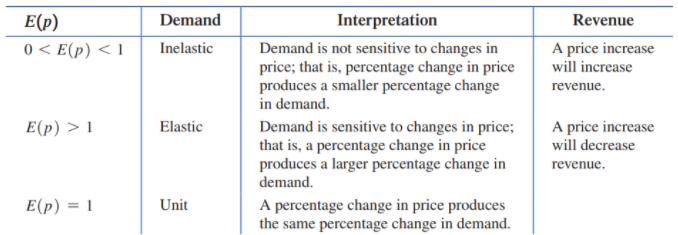
\includegraphics[width=1.0\linewidth]{10-7-1}
\\
\begin{figure}[h!]
	\caption{Revenue and elasticity}
	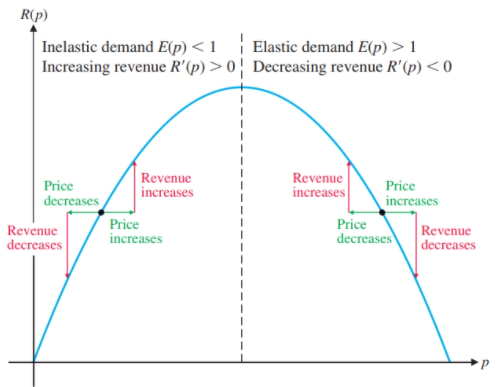
\includegraphics[width=0.8\linewidth]{10-7-2}
\end{figure}
\\ \\

\subsubsection{Examples}
A tie-dye company sells a basic t-shirt for \$12 per shirt. If the price demand equation is
$$x+300p = 9,000$$
Will revenue increase or decrease if the price of a shirt is increased? What shirt price would you recommend to maximize revenue?

\textbf{Solution:}
\begin{align*}
	x = f(p) &= 9,000 -300p = 300(30 -p) \\
	f'(p) &= -300 \\\\
	E(p) &= -\frac{pf'(p)}{f(p)} = -\frac{-300p}{300(30-p)}\\
	&= \frac{p}{30-p} \\\\
	E(13) &= \frac{12}{30-12} = 12/18 = 2/3
\end{align*}
Since $E(13) = 2/3 < 1$, this is inelastic demand and the price may be increased to increase revenue.

Unit elasticity is the point at which changes in price have no effect on revenue. So target your price to get unit elasticity.
\begin{align*}
	E(p)& = \frac{p}{30-p} =1 \\
	p &= 30 -p \\
	2p &= 30 \\
	p &= \$15
\end{align*}
\cleardoublepage
\begin{flalign*}
	&\text{(36) } x =f(p) = 8400 - 7p^2& \tag{Find E(p)}
\end{flalign*}
\begin{align*}
	E(p) &= -\frac{pf'(p)}{f(p)} \\
	&= -\frac{(p)(-14p)}{8400 - 7p^2} \\
	&=\frac{14p^2}{8400 - 7p^2}
\end{align*}

\begin{flalign*}
	&\text{(56) } p +0.004x = 32; &0 \leq p\leq 32& & \tag{Find inelastic demand}
\end{flalign*}
\begin{align*}
	f(p)  &= x= -250(p -32)  \\
	&= 250(32-p)  \\
	E(p) &= -\frac{pf'(p)}{f(p)} \\
	&= -\frac{(p)(-250)}{250(32-p)} = \frac{p}{32-p}
\end{align*}
\indent For which values of p is $0<E(p)<1$? When $p < 32 - p$.
\begin{align*}
	p &<32 -p \\
	2p &< 32 \\
	0 &< p < 16
\end{align*}



\noindent\rule{\textwidth}{1pt}
{\footnotesize Copyright (C) 2021 Garold Dalton --- Released under GNU General Public License v3.0}


\cleardoublepage



\end{document}
